\documentclass[11pt,a4paper,dvipdfmx,titlepage,uplatex]{jsarticle}

\usepackage{ascmac}
\usepackage{url}
\usepackage{amssymb}
\usepackage{comment}
\usepackage{amsthm}
\usepackage{amsmath}

\usepackage[dvipdfmx]{hyperref}
\usepackage{pxjahyper}
\setcounter{tocdepth}{3}%目次をサブセクションまで表示

\bibliographystyle{abbrv}


\newtheoremstyle{mystyle}%   % スタイル名
    {}%b                     % 上部スペース
    {}%                      % 下部スペース
    {\normalfont}%              % 本文フォント
    {}%                      % 1行目のインデント量
    {\bfseries}%             % 見出しフォント
    {.}%                     % 見出し後の句読点
    { }%                     % 見出し後のスペース
    {\thmname{#1}\thmnumber{ #2}\thmnote{ (#3)}}

\theoremstyle{mystyle}
\newtheorem{mythm}{定理}[section]

\makeatletter
\renewenvironment{proof}[1][\proofname]{\par
  \pushQED{\qed}%
  \normalfont \topsep6\p@\@plus6\p@\relax
  \trivlist
  \item\relax
  {\bfseries
  #1\@addpunct{.}}\hspace\labelsep\ignorespaces
}{%
  \popQED\endtrivlist\@endpefalse
}
\makeatother

\usepackage{algorithm,algorithmic}

\usepackage{pdfpages}
\usepackage{graphicx}

\usepackage{mathtools}
\mathtoolsset{showonlyrefs=true}

\usepackage{enumerate}
\usepackage{tabularx}
\newcolumntype{Y}{&gt;{\centering\arraybackslash}X} %中央揃え

\usepackage{booktabs}
\usepackage{siunitx}
\usepackage{dcolumn}
\usepackage{longtable}
\usepackage{wrapfig}
\usepackage{colortbl}
\usepackage{arydshln}

\usepackage{afterpage}%
\usepackage{float}
\usepackage{here}

\usepackage{environ}
\NewEnviron{resizealign}{\sbox0{\let\notag=\relax
		$\begin{matrix}\displaystyle\BODY\end{matrix}$}%
	\sbox1{$(\theequation)$}%
	\sbox2{\parbox{\dimexpr \wd0 + 2\wd1}%
		{\begin{align}\BODY\end{align}}}% for testing
	\noindent\resizebox{\textwidth}{!}{\usebox2}%
}

\usepackage{listings}
\renewcommand{\lstlistingname}{List}
% basicstyle=\ttfamily\small,numberstyle=\ttfamily\footnotesize, numbers=left, frame=single
\lstset{
	% language=c,
	breaklines = true,
	basicstyle=\ttfamily\small,
	commentstyle=\textit,
	% classoffset=1,
	keywordstyle=\bfseries,
	frame=single,
	framesep=5pt,
	showstringspaces=false,
	numbers=left,
	stepnumber=1,
	upquote = true,
	numberstyle=\ttfamily\footnotesize
	% tabsize=2
}

\usepackage{color}
\newcommand{\blue}[1]{\begin{color}{blue}#1\end{color}}
\newcommand{\red}[1]{\begin{color}{red}#1\end{color}}
\newcommand{\green}[1]{\begin{color}{green}#1\end{color}}
\newcommand{\memoblue}[1]{\ifmymemo \begin{color}{memoblue}#1\end{color}\fi}
\newcommand{\modify}[2]{\begin{color}{red}\underline{#1}{#2}\end{color}}

\newcommand{\st}{\textrm{s.t.}}
\newcommand{\Tr}{\mathbf{T}}
\newcommand{\0}{\mathbf{0}}
\newcommand{\diag}{\mathrm{diag}}
\newcommand{\argmin}{\mathrm{argmin}}
\newcommand{\argmax}{\mathrm{argmax}}
\newcommand{\ST}{\mathrm{ST}}
\newcommand{\prox}{\mathrm{prox}}

\newtheorem*{theorem*}{定理}
\newtheorem{theorem}{定理}
\newtheorem{proposition}[theorem]{Proposition}
\newtheorem*{proposition*}{Proposition}
\newtheorem{remark}[theorem]{注}
\newtheorem{example}[theorem]{例}
\newtheorem*{remark*}{注}
\newtheorem{lemma}[theorem]{補題}
\newtheorem{assumption}[theorem]{仮定}
\newtheorem{corollary}[theorem]{系}
\newtheorem{definition}[theorem]{定義}
\newtheorem*{definition*}{定義}

\def\br{\hfill\break}
\def\bold#1{\mbox{\boldmath $#1$}}

%
%file name = bflatex.tex
%
\def\0{\mbox{\bf 0}}
\def\1{\mbox{\bf 1}}
\def\2{\mbox{\bf 2}}
\def\3{\mbox{\bf 3}}
\def\4{\mbox{\bf 4}}
\def\5{\mbox{\bf 5}}
\def\6{\mbox{\bf 6}}
\def\7{\mbox{\bf 7}}
\def\8{\mbox{\bf 8}}
\def\9{\mbox{\bf 9}}
\def\a{\mbox{\boldmath $a$}}
\def\b{\mbox{\boldmath $b$}}
% curled charcter can be used by \chige{a}
\let\chige\c

\def\c{\mbox{\boldmath $c$}}

% details are written in  /usr/share/texmf/tex/plain/base/plain.tex
% \newdimen\zhige \zhige=0pt
% \def\chige#1{{\setbox\zhige\hbox{#1}\ifdim\ht\zhige=1ex\accent24 #1%
%  \else\ooalign{\unhbox\zhige\crcr\hidewidth\char24\hidewidth}\fi}}

\def\cc{\mbox{\boldmath $c$}}
\def\d{\mbox{\boldmath $d$}}
\def\e{\mbox{\boldmath $e$}}
\def\f{\mbox{\boldmath $f$}}
\def\g{\mbox{\boldmath $g$}}
\def\h{\mbox{\boldmath $h$}}
\def\i{\mbox{\boldmath $i$}}
\def\j{\mbox{\boldmath $j$}}
\def\k{\mbox{\boldmath $k$}}
\def\l{\mbox{\boldmath $l$}}
\def\m{\mbox{\boldmath $m$}}
\def\n{\mbox{\boldmath $n$}}
\def\o{\mbox{\boldmath $o$}}
\def\p{\mbox{\boldmath $p$}}
\def\q{\mbox{\boldmath $q$}}
\def\r{\mbox{\boldmath $r$}}
\def\s{\mbox{\boldmath $s$}}
\def\t{\mbox{\boldmath $t$}}
\def\u{\mbox{\boldmath $u$}}
\def\v{\mbox{\boldmath $v$}}
\def\w{\mbox{\boldmath $w$}}
\def\x{\mbox{\boldmath $x$}}
\def\y{\mbox{\boldmath $y$}}
\def\z{\mbox{\boldmath $z$}}
\def\A{\mbox{\boldmath $A$}}
\def\B{\mbox{\boldmath $B$}}
\def\C{\mbox{\boldmath $C$}}
\def\D{\mbox{\boldmath $D$}}
\def\E{\mbox{\boldmath $E$}}
\def\F{\mbox{\boldmath $F$}}
\def\G{\mbox{\boldmath $G$}}
\def\H{\mbox{\boldmath $H$}}
\def\I{\mbox{\boldmath $I$}}
\def\J{\mbox{\boldmath $J$}}
\def\K{\mbox{\boldmath $K$}}
\def\L{\mbox{\boldmath $L$}}
\def\M{\mbox{\boldmath $M$}}
\def\N{\mbox{\boldmath $N$}}
\def\O{\mbox{\boldmath $O$}}
\def\P{\mbox{\boldmath $P$}}
\def\Q{\mbox{\boldmath $Q$}}
\def\R{\mbox{\boldmath $R$}}
\def\S{\mbox{\boldmath $S$}}
\def\T{\mbox{\boldmath $T$}}
\def\U{\mbox{\boldmath $U$}}
\def\V{\mbox{\boldmath $V$}}
\def\W{\mbox{\boldmath $W$}}
\def\X{\mbox{\boldmath $X$}}
\def\Y{\mbox{\boldmath $Y$}}
\def\Z{\mbox{\boldmath $Z$}}
\def\AC{\mbox{$\cal A$}}
\def\BC{\mbox{$\cal B$}}
\def\CC{\mbox{$\cal C$}}
\def\DC{\mbox{$\cal D$}}
\def\EC{\mbox{$\cal E$}}
\def\FC{\mbox{$\cal F$}}
\def\GC{\mbox{$\cal G$}}
\def\HC{\mbox{$\cal H$}}
\def\IC{\mbox{$\cal I$}}
\def\JC{\mbox{$\cal J$}}
\def\KC{\mbox{$\cal K$}}
\def\LC{\mbox{$\cal L$}}
\def\MC{\mbox{$\cal M$}}
\def\NC{\mbox{$\cal N$}}
\def\OC{\mbox{$\cal O$}}
\def\PC{\mbox{$\cal P$}}
\def\QC{\mbox{$\cal Q$}}
\def\RC{\mbox{$\cal R$}}
\def\SC{\mbox{$\cal S$}}
\def\TC{\mbox{$\cal T$}}
\def\UC{\mbox{$\cal U$}}
\def\VC{\mbox{$\cal V$}}
\def\WC{\mbox{$\cal W$}}
\def\XC{\mbox{$\cal X$}}
\def\YC{\mbox{$\cal Y$}}
\def\ZC{\mbox{$\cal Z$}}

\def\Real{\mbox{$\mathbb{R}$}}
\def\Complex{\mbox{$\mathbb{C}$}}
\def\SMAT{\mbox{$\mathbb{S}$}}
\def\Integer{\mbox{$\mathbb{Z}$}}
\def\Natural{\mbox{$\mathbb{N}$}}
\def\ascript{\mbox{\scriptsize $\a$}}
\def\blambda{\mbox{\boldmath $\lambda$}}
\def\etab{\mbox{\boldmath $\eta$}}
\def\balpha{\mbox{\boldmath $\alpha$}}
\def\bbeta{\mbox{\boldmath $\beta$}}
\def\bzeta{\mbox{\boldmath $\zeta$}}
\def\bmu{\mbox{\boldmath $\mu$}}

\newcommand{\oz}{\overline{z}}
\newcommand{\oc}{\overline{\c}}
\newcommand{\ob}{\overline{\b}}
\newcommand{\cO}{\mathcal{O}}
\title{{\large 令和4年度 学士論文}\\ \vskip\baselineskip
taitoru\\タイトル}
\author{東京工業大学 情報理工学院 数理・計算科学系\\
学籍番号 19B31048\\
脇田康平\\
指導教員 山下 真 教授\\
}
\date{2022年2月27日}
\begin{document}

\maketitle

\tableofcontents
\clearpage

\section{はじめに}\label{sec:introduction}
% 研究の大まかな内容
% 研究の意義
% 論文の構成

本論文の構成は以下である。
第\ref{sec:preliminaries}節では、二次錐計画問題(SOCP)に関する前提知識として二次錐計画問題と内点法アルゴリズム、中心パスなどについて説明をする。
第\ref{sec:Deformation_relax_and_penalty}節では、緩和法とペナルティ法に基づく変形について説明する。
第\ref{sec:Numerical_Experience}節では、数値実験を行った結果を示し、各手法の評価を行う。
第\ref{sec:Conclusion}節で、まとめを行う。

\subsection{記法}\label{sec:notation}


この論文で扱う記法を述べる。
\begin{itemize}
  \item $\|\cdot\|$はユークリッドノルムとする。
  \item 行列$\A \in \Real^{k \times m} , \B \in \Real^{k \times n}$を横方向につなげてできる新たな行列$\C \in \Real^{k \times (m+n)}$を
  $ \C = (\A, \B)$ と表記する。
  \item 行列$\A \in \Real^{m \times k} , \B \in \Real^{n \times k}$を縦方向につなげてできる新たな行列$\C \in \Real^{(m+n) \times k}$を
$    \C = (\A ; \B)$ と表記する。
  \item 上付き添え字 $T$ は行列やベクトルの転置を示す。
  \item $\x^T \y$はベクトル$\x,\y \in \Real^n$の内積$\sum_{i=1}^n x_i y_i$である。
  \item 2つのベクトル$\x , \y \in \Real^n$に対して、$\x \circ \y$を次のように定義する。\\
$\x \circ \y = \left(
  \begin{array}{c}
    \x^T \y \\
    x_0 y_1 + y_0 x_1 \\
    \vdots \\
    x_0 y_n + y_0 x_n
  \end{array} \right)
  $
  \item 2つの行列$\A , \B$に対して$\A \oplus \B =
  \begin{pmatrix}
    \A & \0 \\
    \0 & \B \\
  \end{pmatrix}$
  \item $n$次元のベクトル$\e \in \Real^n$かつ、$1$番目の要素のみが$1$で、その他の要素は全て$0$であるベクトルを$\e_n = (1 ; \0)$と表す。
  \item 対角成分以外は0で、対角成分は1行目が$1$,それ以外が$-1$である行列を$\R_n \in \Real^{n \times n}$とする。
  $
  \R_n =
  \begin{pmatrix}
    1 & 0 & \cdots & 0 \\
    0 & -1 & \cdots & 0 \\
    \vdots & \vdots & \ddots & \vdots \\
    0 & 0 & \cdots & -1 \\
  \end{pmatrix}
  $
\end{itemize}

\clearpage

\section{先行研究}\label{sec:preliminaries}
% MISOCPで定義する論文と焼きなましの論文の二つを紹介する。

\section{問題設定}\label{sec:Second_Order_Cone_Programming_without_interiorpoint}
\subsection{対象とする問題について}\label{sec:problem_settings}
本研究が対象とするCVTSPWT(Carrier Vehicle Travering Salesman Problem with Time Window)についての説明を与える。\\
この問題では、速度$V_c$であるcarrierと 速度$V_v$であるvehicleの二つの輸送機器を用いる。ただし, $V_c< V_v$\\
CVTSPWTとは以下の条件を満たすcarrierの経路のうち、スタート地点($q_s$)からゴール地点($q_f$)まで最も少ない時間で航行できる経路とその時間を求める問題である。\\
0. どの目的地にも少なくとも一回訪れる。その際、訪れるのはvehicleでもcarrierでも良い\\
1. ある目的地iには$(u_{i1}, u_{i2})$の間の時間に訪れる。\\
2. vehicleには一度に航行できる距離$a$があり、これを超えてはいけない。航行可能距離は、carrierと同じ座標に来たら再び$a$に戻る。\\
4. vehicleはcarrierから離陸して着陸するまでの間に一箇所しか訪れられない。


\subsection{混合整数二次錐計画問題}\label{sec:Second_Order_Cone_Programming}

まずは、混合整数二次錐計画問題の定義について述べる。\\
% Kを用いた定義
%TODO:
本論文ではこれをユークリッドノルムを用いた以下の形に変形して用いる。
% 変形した最適化問題の定義
\begin{align}
	\begin{array}{rcl}
		\min & : & \f ^T\x \\
		\text{subject to} & : &||\A_i x +\b_i||_2 \leq \c_i^T\x+\d_i, i = 1,\dots, m \\
		& & \F\x=\g\\
		& & \x_i \in \mathbb{Z}, (i=1,\dots, n)
	\end{array}
\end{align}
ここで、$f \in \Real^n , \A, \b, \c, \d$が定数で$x \in \Real^n$が目的変数である。
% 混合整数の場合の定式化
% 混合整数の場合、内点法などのSOCで使えるアルゴが使用できないことを説明
SOCPは目的変数が連続であるため内点法などで最適値を求められるが、MISOCPは変数が離散であるため組合せ最適化のアルゴリズムを用いて最適値を求める必要がある。
\subsection{MISOCPとして定式化}\label{sec:Deformation_relax}
% cplexの解法は数値実験章で比較するのみ
% 誰の既存研究の結果を用いているかを必ず明記する。
ここでは、対象問題を解くためのモデルをMISOCPを用いて定式化する。これは、上でのべた先行研究の拡張である。\\
まずは定数を定義する。\\
	\begin{description}
	\item[$n$]number of target points
	\item[$q_i$] set of target points coodinates
	\item[$q_{min}$] vector of the minimum of the $q_i$
	\item[$q_{max}$]  vector of the maximum of the $q_i$
	\item[$V_v$] vehicle speed
	\item[$V_c$] carrier speed
	\item[$a$] vehicle operational range
	\item[$p_o$]coordinates of the starting point of the trajectory
	\item[$p_f$]coordinates of the ending point of the trajectory
\end{description}
次に決定変数を定義する。
	\begin{description}
	\item[$Q_i$] coodinates in the i th target point to be visited
	\item[$w_{ij}$] binary variables taking 1 if target point j is visited in position j
	\item[$p_{to, i}$] coordinates of the takeoff point for the visit of $Q_i$
	\item[$p_{l, i}$] coorinates of the landing point after the visit of $Q_i$
	\item[$t_{i,1}$] time taken by the vehicle from $p_{to, i}$ to reach $Q_i$
	\item[$t_{i,2}$] time taken by the vehicle from$Q_i$to reach $p_{l, i}$
	\item[$t_i$] time taken by the carrier from $p_{to, i}$  to reach $p_{l, i}$
	\item[$T_1$] time take by the carrier from $p_o$to reach  $p_{to, 1}$
	\item[$T_i$] time take by the carrier from $p_{l, i-1}$to reach  $p_{to, i}$
	\item[$T_{n+1}$] time take by the carrier from $p_{l,n}$to reach  $p_{f}$
	%TODO: uの定義
\end{description}
 MISOCPモデルを定義する。\\
 \begin{align}
 	\begin{array}{rcl}
 		\min & : & \sum_{i=1}^{n}t_i+\sum_{i=1}^{n+1}T_i\\
 		\text{subject to} & : &\|\A_i x +\b_i\|_2 \leq \c_i^T\x+\d_i, i = 1,\dots, m \\
 		& & \F\x=\g\\
 		& & \x_i \in \mathbb{Z}, (i=1,\dots, n)
 	\end{array}
 \end{align}

\section{提案手法}\label{sec:SimulatedAnnealing}
\subsection{焼きなまし法の定義}

焼きなまし法(Simulated Annealing)とは、大域的最適解を求めるためのメタヒューリスティクスの一種である。 局所的最適解を避けるために、目的関数値が一時的に悪くなるような状態へも遷移するという特徴がある。
\subsection{提案手法}
% ヒューリスティックを強調した章の名前にしてもいいかも
% 問題を2ステップに分けて考える。辿る順番を求めるパートと、位置を決めるパート
% 辿る順番を決めるのにSAを用いる
% 辿る順番は組合せ最適化問題であり、選び方が途方もなくあるため全部見るのは困難
% よってこのパートはヒューリスティックを用いて克服する
% 初期回の生成を緩和問題をソルバーで解くことにより効率化できる旨も記す。
%
\section{数値実験}\label{sec:Numerical_Experience}
この節では、前節で導入した
\eqref{NoinnerpointSOCP},\eqref{NoinnerpointSOCP:penalty},\eqref{NoinnerpointSOCP:relax}
の3つのモデルで内点のないSOCPを求解し、数値的に比較を行う。
ここでは、SOCPを解くソルバーとして
SDPT3-4.0~\cite{toh2012implementation}を用いた。
詳しい数値実験の実行環境は表\ref{table:Execution_environment}の通りである。
\begin{table}[hbtp]
  \caption{実行環境}
  \label{table:Execution_environment}
  \centering
  \begin{tabular}{|c|c|}
    \hline
    プロセッサ  & 1.6 GHz デュアルコアIntel Core i5 \\
    \hline
    メモリ  & 8 GB 2133 MHz LPDDR3 \\
    \hline
    OS  & macOS Big Sur バージョン11.6 \\
    \hline
    実装言語  &  MATLAB\_R2021b \\
    \hline
    ソルバー & SDPT3-4.0 \\
    \hline
  \end{tabular}
\end{table}

\subsection{定数の設定}\label{sec:Deformation_to_SDPT3solver}
今回使用したSDPT3では、次のような形式が入力形式であるため、この形式に沿うように入力をする必要がある
%\modify{。~\cite{toh2012implementation}。}{
\cite{toh2012implementation}。
%}
\begin{align}
  \begin{array}{rcll}
    \min & : & \displaystyle{\sum_{j=1}^{n_s}} \left[
    \langle c_j^s , x_j^s \rangle - v_j^s \text{log det}  (x_j^s)
     \right] & + \ \displaystyle{\sum_{i=1}^{n_q}} \left[
     \langle c_i^q , x_i^q \rangle - v_i^q \text{log det}  (x_i^q)
      \right] \\
      & & + \langle c^l , x^l \rangle \ -
      \ \displaystyle{\sum_{k=1}^{n_l}} v_k^l \text{log} x_k^l & + \ \langle
       c^u , x^u \rangle \\
    \text{subject to} & : & \displaystyle{\sum_{j=1}^{n_s}} A_j^s (x_j^s) + \ \displaystyle{\sum_{j=1}^{n_q}} A_j^q (x_j^q) & + \ A^l x^l + \ A^u x^u = b \\
    & & x_j^s \in \KC_s^{s_j} \ \forall j \ , \ x_i^q \in \KC_q^{q_i} \ \forall i , & x^l \in \KC_l^{n_l} \ , \ x^u \in \Real^{n_u} \\
  \end{array}
\end{align}

この問題に対応する双対問題は以下の問題である。
\begin{align}
  \begin{array}{rcll}
    \min & : & \displaystyle{\sum_{j=1}^{n_s}} \left[
    \langle c_j^s , x_j^s \rangle - v_j^s \text{log det}  (x_j^s)
     \right] & + \ \displaystyle{\sum_{i=1}^{n_q}} \left[
     \langle c_i^q , x_i^q \rangle - v_i^q \text{log det}  (x_i^q)
      \right] \\
      & & + \langle
      c^l , x^l
       \rangle \ - \ \displaystyle{\sum_{k=1}^{n_l}} v_k^l \text{log} x_k^l & + \ \langle
       c^u , x^u \rangle \\
  \end{array}\\
  \begin{array}{lllllllll}
    \text{subject to} & : & (A_j^s)^T y & + & z_j^s & = & c_j^s, & z_j^s \in \KC_s^{s_j} & (j = 1,...,n_s) \\
    & & (A_i^q)^T y & + & z_i^q & = & c_i^q, & z_i^q \in \KC_q^{q_i} & (i = 1,...,n_q) \\
    & & (A^l)^T y & + & z^l & = & c^l, & z^l \in \KC_l^{n_l} & \\
    & & (A^u)^T y &   &     & = &  c^u, & y \in \Real^m & \\
  \end{array}
\end{align}

ここで、$x = (x_1^s , \dots , x_{n_s}^s , x_1^q , \dots , x_{n_q}^q , x^l)$,
ただし$x_1^s , \dots , x_{n_s}^s$は対称行列,
$x_1^q , \dots , x_{n_q}^q , x^l$はベクトル
%\modify{}{である}。
である。

一般に
$K$を自己双対なユークリッド空間上の閉凸錐、$A:X \to \Real^m$を線形写像、
$A^*$を$A$の随伴行列、$b \in \Real^m$、$c \in X$とする。
これらを用いるとソルバーの入力標準形は、以下の形式で簡潔に表すこともできる。
\begin{align}
	\label{eq:SDPT3-input}
  \begin{array}{rcc}
    \min & : & \langle \c , \x \rangle \\
    \text{subject to} & : & \x \in \KC \\
    & & \A \x = \b
  \end{array} & \quad
  \begin{array}{rcc}
    \max & : & \b^T \y \\
    \text{subject to} & : & \z \in \KC \\
    & & \A^* \y + \z = \c
  \end{array}
\end{align}

今回のSOCP
\eqref{NoinnerpointSOCP},\eqref{NoinnerpointSOCP:penalty},\eqref{NoinnerpointSOCP:relax}
をソルバーに入力するするためには、上記の形に変形する必要がある。
まず、目的関数に関しては内積以外を$0$に設定すれば良い。
制約は、二次錐制約に関しては$z_i^q \in \KC_q^{q_i}$、
不等式制約に関しては$z^l \in \KC_l^{n_l}$を用いる。%等式制約に関しては$y \in \Real^m$を使う。

例えば、\eqref{NoinnerpointSOCP}を入力するためには、
双対問題を対象として以下のように設定をする。
まず、変数は全てSDPT3の$\y$で扱うこととし、$\y = \x$とする。
次に、不等式制約は二次錐制約として対応させる。
具体的には、不等式制約$\c_i^T \x + d_i \ge \|\A_i \x + \b_i\|$は
\begin{align}
  \begin{pmatrix}
    - \c_i^T \\
    - \A_i \\
  \end{pmatrix}
  \x + \z_i^q =
  \begin{pmatrix}
    d_i \\
    \b_i \\
  \end{pmatrix} , \z_i^q \in \KC_q^{q_i} \ (i = 1 , \dots , m)
\end{align}
の形に変形することで、$(A_i^q)^T y + z_i^q = c_i^q, z_i^q \in \KC_q^{q_i} (i = 1,...,n_q)$の二次錐制約に対応させる。
また、等式制約$\F \x = \g$は
$A^u = \F^T , c^u = \g_u$として
\begin{align}
  (A^u)^T y = c^u
\end{align}
の制約に対応させる。
同様の手順により\eqref{NoinnerpointSOCP:penalty},\eqref{NoinnerpointSOCP:relax}も
SDPT3に入力可能である。

\subsection{初期点とパラメータの設定}\label{sec:parameter_settings}

SDPT3は以下のような引数をとる。
\begin{center}
  \text{[obj,X,y,Z,info,runhist] = sqlp(blk,At,C,b,OPTIONS,X0,y0,Z0)}
\end{center}
ここで、blkはSOCPの錐を表すブロック構造のセル配列、
At, C, b はSOCPの入力行列などを表す。また、
OPTIONSはSDPT3が用いるパラメータであり、
X0 , y0 , Z0は内点法の初期点を表す。

今回の数値実験では、OPTIONS,X0,y0,Z0はSDPT3が設定するデフォルト値を用いた。
特に、デフォルトの場合のy0の初期点は、次のように$(-1,1)$から発生する$n$次元正規分布乱数ベクトルで設定される。
\begin{align}
  y0 = \text{randn}(n,1)
\end{align}

得られた最適解の精度を評価するために、いくつかの定義を行う。まず、
\begin{align}
  \lambda_{\min,\KC} (\x) = \min \left\{ \underset{j=1,\cdots,n_s}{\min} \lambda_{\min} (x_j^s) , \underset{k=1,\cdots,n_q}{\min} \lambda_{\min,q} (x_k^q) , \underset{h}{\min} (x_h^l) \right\}
\end{align}
とする。ここで、あるベクトル$\a = (a_1 ; \overline{\a})$に対して
$\lambda_{\min,q} (\a) = a_1 - \|\overline{\a}\|_2$,
ある対称行列$\A$に対して$\lambda_{\min} (\A) = \A$の最小の固有値とする。
また、ベクトル$\x = (x_1 , \cdots , x_n) , \z = (z_1 , \cdots , z_n) \in \Real^n$に対して、
$\|\x\|_1 = \underset{i=1,\cdots,n}{\max} |x_i|$,
$\langle \c,\x \rangle = \c^T \x$
とする。
これらを踏まえて、以下の6つを定義する。
これらはDIMACS error~\cite{mittelmann2003independent}とも呼ばれる。
\begin{align}
			\text{error1} &= \frac{\|\A \x - \b\|}{1 + \|\b\|_1} &
			\text{error2} &= \max \{ 0, - \frac{\lambda_{\min , \KC} (\x)}{1 + \|\b\|_1} \} \\
			\text{error3} &= \frac{\|\A^* \y + \z - \c\|}{1 + \|\c\|_1} &
			\text{error4} &= \max \{ 0, - \frac{\lambda_{\min , \KC} (\z)}{1 + \|\b\|_1} \} \\
			\text{error5} &= \frac{\langle \c,\x \rangle - \b^T \y}{1 + \langle \c,\x \rangle + \b^T \y} &
			\text{error6} &= \frac{\langle \x,\z \rangle}{1 + \langle \c,\x \rangle + \b^T \y}
\end{align}
これらのDimacs errorには、以下の性質があることが知られている。
\begin{itemize}
  \item error2とerror4は、得られた解のうち$\x , \z \in \KC$であるならば、ともに0をとる。
  よって、得られた解の中で$\x,\z$が二次錐制約を満たしているかどうかは、error2とerror4の数値で確認することができる。
  \item 得られた解のうち$\x , \z \in \KC$が実行可能な場合、厳密な計算式では
  error5 $=$ error6となる。しかし、ソルバーで出力される解は数値誤差を含むので、必ずしも一致するとは限らない。
  \item error5は双対ギャップを表しており、出力された解が厳密に実行可能解であれば弱双対定理より$0$以上である。しかし、数値誤差の影響により、error5は負の値となる可能性がある。
\end{itemize}

これらを用いると、閾値を$\epsilon>0$としたときの
SDPT3の終了条件は以下のように示すことができる。
\begin{center}
  終了条件: \ $\max\{\text{error}1, \text{error}2, \dots, \text{error}6\} < \epsilon$
\end{center}
この条件を満たすまで、探索方向による計算を続け、条件を満たした時点で、その点を最適解として出力し、反復を終了する。
なお、SDPT3では、デフォルトの閾値は$\epsilon = 10^{-8}$である。

\subsection{テスト問題の生成方法}\label{sec:Problem_Generation}

%\red{\eqref{NoinnerpointSOCP}の$\A, \b, \c$ などを乱数などでどう生成しているかが書かれていない。}

生成する問題\eqref{NoinnerpointSOCP}については非有界であると
数値誤差が非有界に起因するか内点がないことに起因するか判別が困難であるため、
どの問題でも有界制約を追加し、必ず有界な問題となるように設定した。
これにより、必ず最適解が存在するように問題を生成した。

具体的には、まず$i = 1 , \dots , m-1$に対して
$\A_i \in \Real^{n \times n_i}, \b_i \in \Real^n, \c_i \in \Real^{n_i}$
を正規分布からなる乱数を要素に持つ変数として設定する。MATLABでは以下のように設定する。
$\overline{x} = \text{randn} (n,1) \in \Real^n$に対しては
\begin{align}
  A\{i\} &= \text{randn}(n\_i,n) , b\{i\} = \text{randn}(n\_i,1) ,
  c\{i\} = \text{randn}(n,1) , \\
  d\{i\} &= -c\{i\}' \overline{x} + \text{norm}(A\{i\}' \overline{x}+b\{i\}) + 10
\end{align}
とする。このようにすることで、$i = 1 , \dots , m-1$の場合の
不等式制約を満たす変数$\overline{x}$が必ず存在することになる。
次に、$\A_m \in \Real^{n \times n_i}, \b_m \in \Real^{n}, \c_m \in \Real^{n_i}$と、
ある$\overline{\x} \in \Real^{n_i}$が満たすべき不等式制約
$\c_i^T \overline{\x} + d_i \ge \|\A_i \overline{\x} + \b_i \|$に対して、
$\A_m = \I_m, \b_m = \0, \c_i = \0$とすることで、この不等式は
\begin{align}
	\0 + d_m \ge \|\I_m \x + \0\| = \|\x\|
\end{align}
となる。よって、$d_m = \|\overline{\x}\|+1$と設定すれば、
$i=m$の場合の不等式制約は$\|\overline{\x}\|+1 \ge \|\x\|$となるので、有界な問題となる。
この場合、MATLABでは$\overline{x} = \text{randn} (n,1) \in \Real^n$に対して以下のように設定する。
\begin{align}
  A\{m\} = \text{eye}(n) , b\{m\} = \text{zeros}(n,1) ,
  c\{m\} = \text{zeros}(n,1) ,
  d\{m\} = \text{norm} (\overline{x})^2 + 1
\end{align}

\subsection{実験結果}\label{sec:Numerical_Result}
実験結果について、まずは計算時間と精度で評価をし、続いて
反復回数による評価を行う。また、ペナルティ係数の設定が与える影響についても、
検討する。
\subsubsection{計算時間と精度の評価}\label{sec:Evaluation_CPUtime_and_accuracy}

この節では、3手法による計算時間とDimacs error値の違いに着目をする。
表\ref{table:Experimental_Result}は、問題のサイズを変更した場合の各手法で求解までにかかった計算時間とDimacs errorの数値を表している。
問題のサイズを決定する$m,n_i,\overline{m}$の3つを変えて数値実験を行った。
なお、ペナルティ法のペナルティ係数は$10^2$とした。

表\ref{table:Experimental_Result}では、%この表は、6つのブロックに分かれている。
%サイズを6種類に変更して実験を行った。
各ブロックにおいて横の行が各手法に対応しており、
縦の列がそれぞれSDPT3に入力するように変換した後の変数の数、制約の数、計算時間(秒)、Dimacs errorに対応している。
% ここで、計算時間はCPUがかかった全体の時間としている。

%\begin{minipage}
\begin{table}[h]
  \caption{各手法での計算時間とDimacs errorの数値}
  \label{table:Experimental_Result}
  %\centering
  \scriptsize
  %\small
  \begin{tabular}{|c|c|c|c|c|c|c|c|c|c|}
    \cline{1-10}
    \multicolumn{10}{|c|}{$m = 3,n_i = 5,\overline{m}= 3$}\\
    %\hline
    \cline{1-10}
    & 変数の数 & 制約の数 & 計算時間(秒) & error1 & error2 & error3 & error4 & error5 & error6 \\
    %\hline
    \cline{1-10}
    通常の内点法  & 4 & 10 & 0.9 & 1.44E-11 & 0.00E+0 & 3.33E-11 & 0.00E+0 & 5.96E-09 & 6.58E-09 \\
    %\hline
    \cline{1-10}
    ペナルティ法 & 10 & 12 & 1.07 & 4.21E-16 & 0.00E+0 & 1.58E-11 & 0.00E+0 & 5.95E-09 & 7.57E-09 \\
    %\hline
    \cline{1-10}
    緩和法 & 39 & 16 & 1.37 & 9.14E-15 & 0.00E+0 & 3.18E-11 & 0.00E+0 & 7.54E-09 & 9.40E-09 \\
    %\hline
    \cline{1-10}
    \multicolumn{10}{|c|}{$m = 10,n_i = 10,\overline{m} = 10$}\\
    \cline{1-10}
    & 変数の数 & 制約の数 & 計算時間(秒) & error1 & error2 & error3 & error4 & error5 & error6 \\
    %\hline
    \cline{1-10}
    通常の内点法  & 4 & 31 & 1.14 & 1.19E-12 & 0.00E+0 & 1.18E-11 & 0.00E+0 & 8.53E-09 & 8.94E-09 \\
    %\hline
    \cline{1-10}
    ペナルティ法 & 24 & 33 & 1.24 & 4.86E-15 & 0.00E+0 & 3.93E-12 & 0.00E+0 & 4.72E-09 & 5.70E-09 \\
    %\hline
    \cline{1-10}
    緩和法 & 218 & 51 & 2.69 & 2.55E-14 & 0.00E+0 & 1.23E-11 & 0.00E+0 & 5.56E-09 & 7.60E-09 \\
    %\hline
    \cline{1-10}
    \multicolumn{10}{|c|}{$m = 30,n_i = 10,\overline{m} = 20$}\\
    \cline{1-10}
    & 変数の数 & 制約の数 & 計算時間(秒) & error1 & error2 & error3 & error4 & error5 & error6 \\
    %\hline
    \cline{1-10}
    通常の内点法  & 4 & 71 & 2.35 & 5.22E-13 & 0.00E+0 & 6.90E-12 & 0.00E+0 & 7.07E-09 & 7.53E-09 \\
    %\hline
    \cline{1-10}
    ペナルティ法 & 54 & 73 & 3.23 & 1.73E-14 & 0.00E+0 & 3.18E-12 & 0.00E+0 & -1.74E-09 & 6.79E-09 \\
    %\hline
    \cline{1-10}
    緩和法 & 548 & 121 & 6.39 & 5.60E-14 & 0.00E+0 & 6.93E-12 & 0.00E+0 &
    6.34E-09 & 8.53E-09 \\
    %\hline
    \cline{1-10}
    \multicolumn{10}{|c|}{$m = 20,n_i = 20,\overline{m} = 40$}\\
    \cline{1-10}
    & 変数の数 & 制約の数 & 計算時間(秒) & error1 & error2 & error3 & error4 & error5 & error6 \\
    %\hline
    \cline{1-10}
    通常の内点法  & 4 & 101 & 3.19 & 6.54E-12 & 0.00E+0 & 8.07E-12 & 0.00E+0 & 8.57E-09 & 9.78E-09 \\
    %\hline
    \cline{1-10}
    ペナルティ法 & 64 & 103 & 3.96 & 4.07E-14 & 0.00E+0 & 1.49E-12 & 0.00E+0 & 4.45E-09 & 9.26E-09 \\
    %\hline
    \cline{1-10}
    緩和法 & 1248 & 161 & 9.16 & 5.95E-14 & 0.00E+0 & 2.07E-12 & 0.00E+0 & 4.84E-09 & 7.09E-09 \\
    %\hline
    \cline{1-10}
    \multicolumn{10}{|c|}{$m = 50,n_i = 50,\overline{m} = 60$}\\
    \cline{1-10}
    & 変数の数 & 制約の数 & 計算時間(秒) & error1 & error2 & error3 & error4 & error5 & error6 \\
    %\hline
    \cline{1-10}
    通常の内点法  & 4 & 171 & 4.59 & 2.40E-11 & 0.00E+0 & 1.67E-12 & 0.00E+0 & 7.65E-09 & 8.52E-09 \\
    %\hline
    \cline{1-10}
    ペナルティ法 & 114 & 173 & 4.10 & 1.29E-07 & 0.00E+0 & 1.10E-06 & 0.00E+0 & -7.03E-02 & 3.05E-04 \\
    %\hline
    \cline{1-10}
    緩和法 & 5568 & 281 & 48.35 & 9.30E-13 & 0.00E+0 & 6.97E-13 & 0.00E+0 & 6.72E-09 & 9.22E-09 \\
    %\hline
    \cline{1-10}
    \multicolumn{10}{|c|}{$m = 100,n_i = 100,\overline{m} = 80$}\\
    \cline{1-10}
    & 変数の数 & 制約の数 & 計算時間(秒) & error1 & error2 & error3 & error4 & error5 & error6 \\
    %\hline
    \cline{1-10}
    通常の内点法  & 4 & 261 & 6.21 & 2.03E-10 & 0.00E+0 & 3.96E-13 & 0.00E+0 & 5.26E-09 & 5.96E-09 \\
    %\hline
    \cline{1-10}
    ペナルティ法 & 184 & 263 & 6.57 & 2.80E-07 & 0.00E+0 & 2.70E-07 & 0.00E+0 & -3.42E-02 & 6.20E-04 \\
    %\hline
    \cline{1-10}
    緩和法 & 18088 & 441 & 375.38 & 7.75E-13 & 0.00E+0 & 2.69E-13 & 0.00E+0 & 6.32E-09 & 8.02E-09 \\
    %\hline
    \cline{1-10}
  \end{tabular}
\end{table}

表\ref{table:Experimental_Result}から分かるように、
計算時間は、通常の内点法とペナルティ法ではどのサイズの問題でもほぼ同じ計算時間であるが、
緩和法は問題の規模が大きくなるとかなり長い計算時間を要する。
これは、第\ref{sec:Deformation_relax}節で述べたように、生成される変数と制約の数が関係していることが分かる。

次に、error値に着目する。
まず、error2とerror4について検討する。
どの実験結果においてもerror2とerror4が$0$に近い値となっており、全ての手法で実行可能解を求められていることが分かる。

また、等式条件とDimacs errorの対応について考えてみる。
error1は、主問題における等式制約に関する数値誤差、
error3は双対問題における等式制約に関する数値誤差、
つまりどれくらい等式制約から逸脱しているかを表現している。
error1とerror3を見てみると、問題のサイズが小さい場合は、通常の内点法が$10^{-12}$の精度で求解できているのに比べて、ペナルティ法と緩和法は$10^{-14}$という精度で求解を達成できていることがわかる。
次に、問題のサイズが大きい場合に注目すると、
通常の内点法の精度は$10^{-12}$と変わらないままとなっている。
しかし、ペナルティ法は通常の内点法に比べて$10^{-7}$まで精度が落ちてしまっているのに対して、
緩和法はサイズが大きくなっても$10^{-13}$という良い精度を保ちつつ求解ができていることがわかる。

さらに error5, error6 についても考察を与える。
error5は双対ギャップに対応している。
error5を見てみると、通常の内点法と緩和法は$10^{-9}$程度の精度が安定して得られている。
しかし、ペナルティ法では$m = 30,n_i = 10,\overline{m} = 20$と$m = 50,n_i = 50,\overline{m} = 60$および$m = 100,n_i = 100,\overline{m} = 80$の場合に負の値となっている。
定理\ref{theorem:weak-duality}より、本来error5は$0$以上の値を取るはずである。
数値誤差の影響もあり、ペナルティ法では良い解が得られているわけではないことがわかる。
error6 においても、ペナルティ法では精度値が落ちる場合が確認できる。

\subsubsection{反復回数の評価}\label{sec:Evaluation_itertimes}

次に、各手法の求解に要する反復回数で比較を行う。
ここでは、ペナルティ係数を$10^3$ に設定した。
問題のサイズ$m,n_i,\overline{m}$
をそれぞれ$1$〜$100$の範囲でランダムな値として生成した。具体的には
\begin{align}
  m,n_i,\overline{m} = 1 + \text{round}(100*\text{rand})
\end{align}
とした。
その条件の下で、各手法の反復回数を集計しグラフにしたものが
図\ref{figure:hanpukukaisu}
である。
合計50回実験を行い、
横軸が実験番号を表し、縦軸が3手法の反復回数である。

\begin{figure}[h]
  \begin{center}
    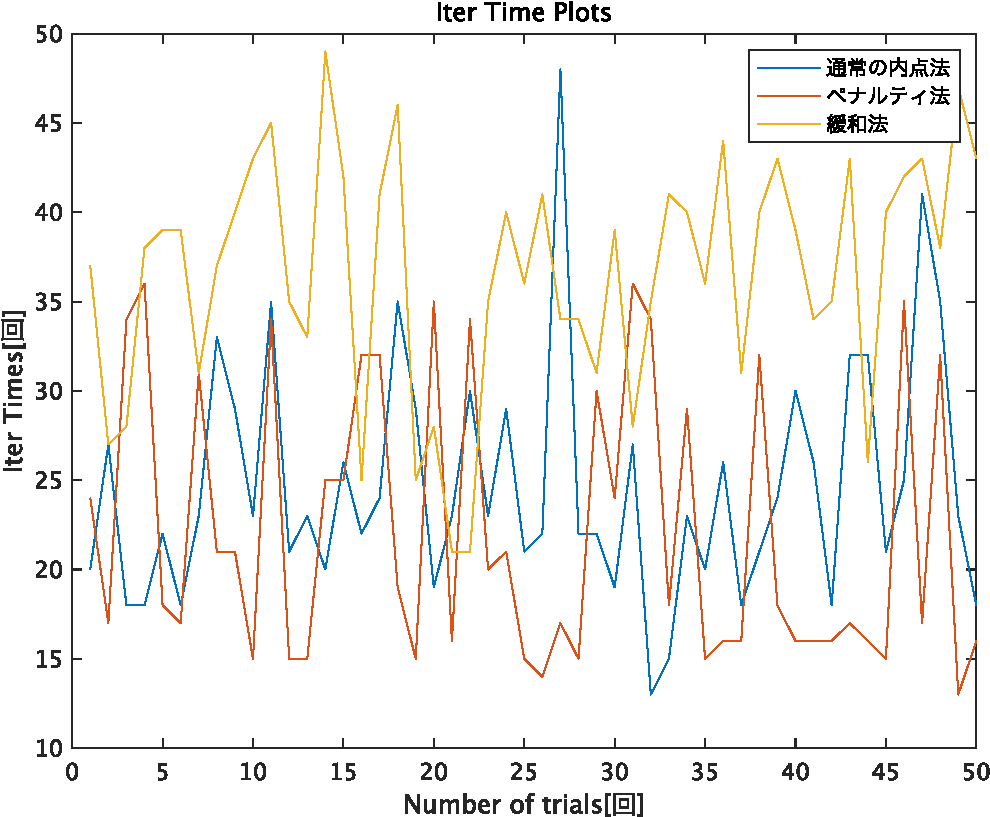
\includegraphics[width=100mm,height=65mm]{IterTimePlots2_1.pdf}
    \caption{各手法の求解に要する反復回数 \label{figure:hanpukukaisu}}
  \end{center}
\end{figure}

平均回数は、通常の内点法が24.6回、ペナルティ法が22.2回、緩和法が36.6回となり、
どの問題においても通常の内点法とペナルティ法に比べて、
緩和法では最適解を求めるのに多い反復回数を必要とする。
%\red{この次の文、前の文と矛盾してます。反復回数が多いのは、緩和法のはず。}
これは、緩和法では決定変数$\y$の数がかなり大きくなるため、他の2手法に比べて
error値の数値誤差が大きく出てしまうため、全てのerror値が$\epsilon$以下となるという反復の終了条件を満たしにくいことが影響していると考えられる。
%ペナルティ法では実行可能領域が広がっているため、中心パスを通って最適解にたどり着くための距離を多く必要とするためだと予想される。
また、大体の場合において若干ペナルティ法の方が通常の内点法に比べて少ない反復回数で
求解できていることがわかる。
これは、ペナルティ法では実行可能領域が広がるため、
通常の内点法に比べてステップ長を少しだけ長く取ることができることが影響していると考えられる。

\subsubsection{yet}\label{sec:Evaluation_penalty_coefficient}

% これ以前に行っていた実験では、ペナルティ係数は全て$10^3$の値に固定していた。
ここでは、ペナルティ係数を$10^1$〜$10^5$の値からランダムに設定することで、
ペナルティ係数の大きさが求解にどのような影響があるのかを調べる。
\ref{sec:Evaluation_itertimes}節と同様に$i = 1 , \cdots , m$に対して
\begin{align}
  P_i,\overline{P}_i = 100 + \text{round}(9900*\text{rand})
\end{align}
で生成した。
計算時間と反復回数をまとめたのが図\ref{figure:CPUtime}のグラフである。

\begin{figure}[tp]
  \begin{center}
    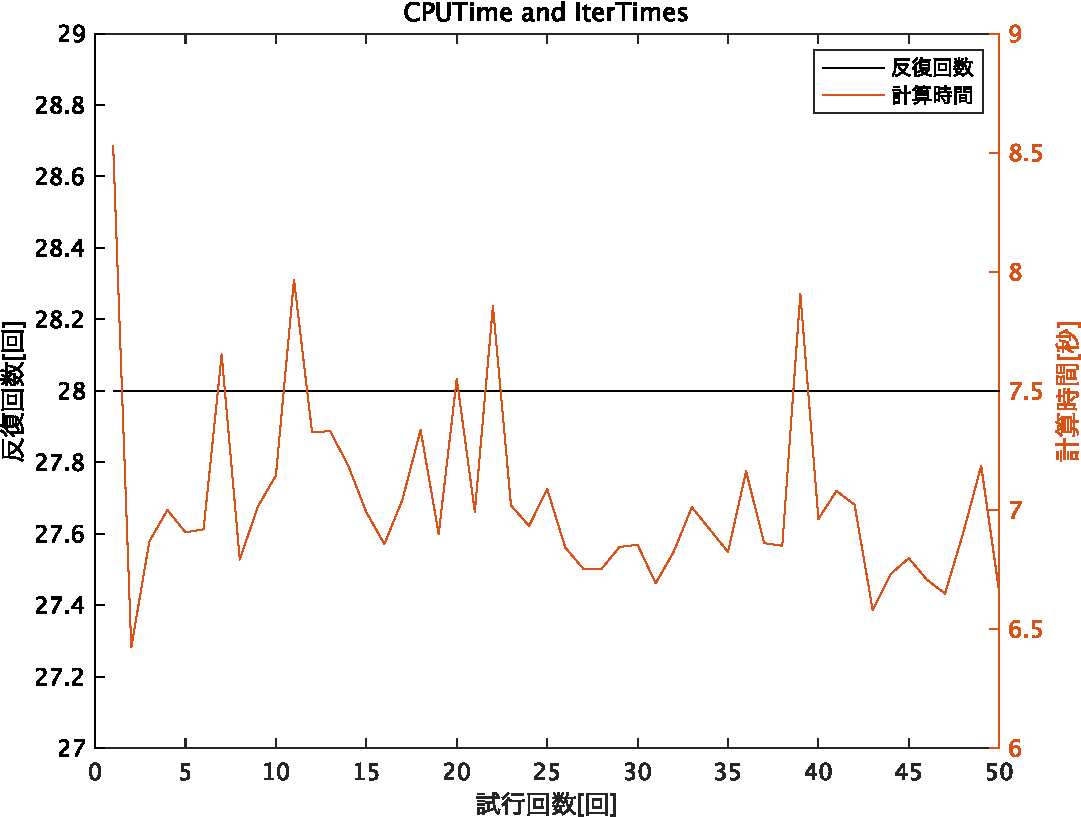
\includegraphics[width=100mm,height = 65mm]{CPUtimePlots5.pdf}
    \caption{CPU計算時間と反復回数 \label{figure:CPUtime}}
  \end{center}
\end{figure}

%\red{図\ref{figure:CPUtime}は右の軸と左の軸で間違っている?反復回数が整数でない
% 状況になっている。}
図\ref{figure:CPUtime}から、以下がわかる。
求解にかかる反復回数は、ペナルティ係数を変化させた場合でも全て同じ28回となった。
また、かかるCPU計算時間は、概ね7秒と変化がなく安定していた。
このことから、ペナルティ係数を変化させたとしても、反復回数と計算時間などに
大きな影響はないことがわかった。
より発展的な実験として、目的関数に追加するペナルティ係数を、
二次関数や対数障壁関数などの異なる関数として追加した場合を考えると、
また違った結果が得られるのではないかと考えられる。

次にペナルティ係数を変化させた場合のDimacs errorへの影響について考察する。
表\ref{table:Experimental_Result_penalty_dimacserror}
は、\eqref{NoinnerpointSOCP:penalty}において
ペナルティ係数を変化させた場合のDimacs errorの数値を表している。
ペナルティ係数の具体的な値としては、先ほどと同様$10^1$〜$10^5$の範囲の中で値を変化させて実験を行った。

\begin{table}[tp]
  \caption{ペナルティ係数を変化させた場合のDimacs errorの数値}
  \label{table:Experimental_Result_penalty_dimacserror}
  \centering
  \scriptsize
  %\small
  \begin{tabular}{|c|c|c|c|c|c|c|}
    \cline{1-7}
    \multicolumn{7}{|c|}{$m = 50,n_i = 50,\overline{m}= 50$}\\
    %\hline
    \cline{1-7}
    & error1 & error2 & error3 & error4 & error5& error6 \\
    %\hline
    \cline{1-7}
    $P, \overline{P} = 10$ & 1.39E-13 & 0.00E+0 & 6.45E-14 & 0.00E+0 & 4.93E-09 & 5.58E-09 \\
    %\hline
    \cline{1-7}
    $P, \overline{P} = 10^2$ & 6.56E-13 & 0.00E+0 & 4.03E-14 & 0.00E+0 & 4.93E-09 & 5.63E-09 \\
    %\hline
    \cline{1-7}
    $P, \overline{P} = 10^3$  & 9.55E-14 & 0.00E+0 & 5.25E-14 & 0.00E+0 & -1.40E-08 & 6.27E-09 \\
    %\hline
    \cline{1-7}
    $P, \overline{P} = 10^4$  & 1.57E-13 & 0.00E+0 & 3.92E-14 & 0.00E+0 & -2.82E-09 & 5.41E-09 \\
    %\hline
    \cline{1-7}
    $P, \overline{P} = 10^5$  & 9.59E-11 & 0.00E+0 & 3.27E-07 & 0.00E+0 & -0.999 & 1.47E-05 \\
    %\hline
    \cline{1-7}
  \end{tabular}
\end{table}

表\ref{table:Experimental_Result_penalty_dimacserror}
からわかるように、error2とerror4がともに0になっていたので、
全ての場合で出力された解は二次錐に含まれている。
$P, \overline{P}$の値に着目すると、$P, \overline{P}$の値が$10^2$以下の場合では、どのerror値も全て0に近い値となっていることから、安定して解を求めることができている。
逆に、$P, \overline{P}$の値が$10^5$のようにかなり大きい場合は、双対ギャップに対応するerror5が負の値となっていることからうまく求解できていないことがわかる。
$P, \overline{P}$の値が$10^3,10^4$の場合は、error5が負の値となっている。
しかし、この数値実験では多少の数値誤差を含むので、
error5がほぼ0に近い値となっていること、および、その他のerror値が$P, \overline{P} = 10,10^2$
の時と同じ精度で正の値かつ0に近い値となっていることから、
安定して求解できていると考えられる。

\subsubsection{yet}
\ref{sec:Deformation_penalty}節で見たように、ペナルティ法では不等式制約に$\xi_i,\overline{\xi}_i$を加えて実行可能領域を広げ、必ず実行可能内点を持つようにすることで数値的安定性の向上を目指した。
ここで、追加した変数$\xi_i,\overline{\xi}_i$に着目し、
追加する前の問題\eqref{NoinnerpointSOCP}と
追加した後の問題\eqref{NoinnerpointSOCP:penalty}で、
どれくらい実行可能領域が変化しているかを考える。

そのために、$\xi_i,\overline{\xi}_i$の値に着目する。
今回は、$m = 10, \overline{m} = 10$として数値実験を行った。
その他は、$n_i = 10 , P = 10^2$と設定した。
以前の実験と同様に有界性も仮定した。
得られた具体的な$\xi_i,\overline{\xi}_i$の値は以下である。
\begin{align}
  \xi =
  \begin{pmatrix}
    2.9638E-12 \\
    2.9665E-12 \\
    2.9633E-12 \\
    2.9655E-12 \\
    2.9687E-12 \\
    2.9638E-12 \\
    2.9643E-12 \\
    2.9649E-12 \\
    2.9666E-12 \\
    2.9597E-12 \\
  \end{pmatrix}
  \ , \ \overline{\xi} =
  \begin{pmatrix}
    3.7917E-12 \\
    3.7649E-12 \\
    3.8559E-12 \\
    3.5737E-12 \\
    3.6003E-12 \\
    3.5165E-12 \\
    3.8981E-12 \\
    4.0037E-12 \\
    3.7935E-12 \\
    4.0776E-12 \\
  \end{pmatrix}
\end{align}

この数値から、各ベクトル$\xi$と$\overline{\xi}$の各成分にばらつきはなく、
ほぼ同じ値となる結果となった。
%\red{この次の文、上の結果と逆のことを書いている?}
また、若干$\overline{\xi}$の成分の方が$\xi$の成分よりも大きい値となった。
具体的な値としては、$10^{-12}$の精度となっていてほぼ0に近い値である。
このことから、最適解の領域はあまり広がらず、元の問題\eqref{NoinnerpointSOCP}
と同じ制約を保ったまま求解できていることがわかる。

%\subsection{(実験結果に対する理論的考察orToh先生にもらったコードの確認)}\label{sec:Consideration_to_Numerical_Expericence}
%どちらか、余裕があればやりたいです。
%\red{間に合わないといけないので、このsubsectionはコメントアウトしましょう。}

\clearpage

\section{結論}\label{sec:Conclusion}
%卒論は適宜バックアップをとっておく!
本論文では、実行可能内点を持たないようなSOCPを内点法で求解する場合に不安定になりやすいことを解消する方法として、
緩和法とペナルティ法を施すことで、数値的安定性の向上を目指した。
第\ref{sec:Numerical_Experience}節の結果から、求解の精度は、
どの問題のサイズに対しても緩和法が他の手法に比べて有効であることがわかった。
逆に、求解にかかる反復回数は、緩和法が他の手法に比べて少し多い回数を必要とする結果となった。
計算時間は、緩和法では変数の数が多くなるため、通常の内点法とペナルティ法に比べて、
求解までに要する計算時間が長くなることが分かった。
また、ペナルティ法のみに着目してペナルティ係数を変化させた場合では、ペナルティ係数を$10^4$以上の値だと安定して求解できない結果となったが、
それより小さい値で設定をすることで良い精度を保ったまま安定して解を求めることができていることが確認された。
求解にかかる反復回数は問題のサイズを変えても同じ回数を要する結果となった。

今後の課題としては、以下が挙げられる。
ペナルティ法による変形について、目的関数に追加するペナルティ項を1次関数で追加したので、
二次関数などの別の関数を使ったペナルティ項を追加して実験をすることが考えられる。
緩和法については、問題のサイズを大きくした際、求解にかかる時間が急激に増えてしまうというデメリットがわかった。緩和法の定式化に基づく効率的な内点法を設計するなどして、求解にかかる時間を短くすることも今後の課題と考えられる。

%\red{このあとの文章は削除しましょう。どういうコードなのかを説明する必要もありますし、今回の内容とどのくらい関係があるかも、まだ調べてないし。} また、SDPT3の作成者であるToh先生からいただいたコードを用いて同様の実験を行い、比較をすることも今後の課題となる。

\clearpage
\section*{謝辞}\label{sec:Acknowledgement}

本論文の執筆にあたり、数多くの助言や論文の添削、さらには数多くの質問に対して優しく丁寧に指導して頂きました指導教員の山下真教授に感謝いたします。
また、ゼミを通じて多くのことを教えてくださった山下研究室、澄田研究室の先生方や先輩方に感謝いたします。
最後に、学士論文をともに取り組んだ山下研究室、澄田研究室の仲間や友人、支えてくださった家族には感謝いたします。


\clearpage
%\red{参考文献のBibファイルは、修正が必要な個所が多かったので修正しておきました。}
\begin{small}
\bibliography{soturon.bib}
\end{small}


\end{document}
